\chapter{Программная реализация платформы для проведения электронных голосований на основе технологии блокчейн}

Платформа для проведения электронных голосований, по описанному в третьей части второй главы протоколу, реализована на описанной в четвертой части второй главы платформе Ethereum в виде смарт-контракта, написанного на языке программирования Solidity.

Для разработки смарт-контракта использовалась среда разработки децентрализованных приложений на платформе Ethereum — Hardhat. Hardhat поставляется в виде NPM пакета для платформы Node.js, решая задачи компиляции, развертывания, тестирования и отладки программного обеспечения. В Hardhat встроена локальная сеть Ethereum, под названием «Hardhat Network», функциональность который сосредоточена на отладке кода написанного на Solidity, включая трассировку стека и явный сообщения об ошибках.

\section{Описание структур данных}

Для хранения информации о кандидате, создана структура \verb|Candidate|, содержащая поля \verb|id| и \verb|name| (листинг \ref{ls:candidate}). Данная структура, включается в контракты \verb|VotePlatform| и \verb|Vote|.

\begin{lstlisting}[caption={Объявление структуры Candidate}, label={ls:candidate}]
struct Candidate {
    uint256 id;
    string name;
}
\end{lstlisting}

Голосования реализованы в виде отдельного контракта, который содержит всю необходимую информацию о каждом голосовании (листинг \ref{ls:votestruct}).

\begin{lstlisting}[caption={Поля контракта Vote}, label={ls:votestruct}]
bool public multipleChoice;
uint public dateOfCreating;
uint public dateOfStart;
uint public dateOfEnd;
uint public dateOfEndAddPrivateKeys;
VotingPlatformLib.Candidate[] public candidates;
uint public votersCount;
uint public modulus;    uint public exponent;
uint[] public verifiedSignature;
Ballot[] public ballots;

struct Ballot {
    address owner;
    bytes encryptedValue;
    bytes privateKey;
    uint dateOfVote;
}
\end{lstlisting}

Контракт \verb|VotingPlatform| содержит в себе массив из контрактов \verb|Vote| и адрес инициализатора контракта, поскольку создавать новые голосования может только владелец платформы.

\section{Описание методов смарт-контрактов}

Создание новых голосований осуществляет через контракт \verb|VotingPlatform|, его метод \verb|createVote| (листинг \ref{ls:createVote}) принимает параметры: \verb|_multipleChoice| — возможен ли выбор нескольких избирателей, \verb|_dateOfStart| — дата начала голосования в формате UNIX, \verb|_dateOfEnd| — дата окончания в формате UNIX, \verb|_dateOfEndAddPrivateKeys| — дата окончания приема приватных ключей, \verb|_candidates| — список кандидатов, за которых можно отдать свой голос, \verb|_votersCount| — количество зарегистрированных избирателей, \verb|_modulus| — первая часть публичного ключа RSA, \verb|_exponent| — вторая часть публичного ключа RSA. После чего, создает новый объект Vote и добавляет его в массив votes, вызывая событие \verb|VoteAdded|. К данному методу добавлен модификатор \verb|OnlyOwner|, который проверяет, что транзакцию инициировал владелец контракта.

\begin{lstlisting}[caption={Создание нового голосования}, label={ls:createVote}]
function createVote(
    bool _multipleChoice,
    uint256 _dateOfStart,
    uint256 _dateOfEnd,
    uint256 _dateOfEndAddPrivateKeys,
    VotingPlatformLib.Candidate[] memory _candidates,
    uint256 _votersCount,
    uint256 _modulus,
    uint256 _exponent
) external onlyOwner {
    votes.push(
        new Vote(
            _multipleChoice,
            _dateOfStart,
            _dateOfEnd,
            _dateOfEndAddPrivateKeys,
            _candidates,
            _votersCount,
            _modulus,
            _exponent
        )
    );
    emit VoteAdded(votes.length - 1);
}
\end{lstlisting}

Для работы функции \verb|pushBallot|, которая отвечает за добавление выбора избирателя, реализовано четыре модификатора (листинг \ref{ls:modify}). Модификатор в языке Solidity — свертка исходного кода, которая используется для изменения семантики функции декларативным способом. Модификаторы вызываются перед выполнением функции, в них проверяются различные условия, при успешном выполнении которых, функция выполняется. Модификаторы очень полезны, поскольку уменьшают избыточность кода.

\begin{lstlisting}[caption={Модификаторы метода pushBallot}, label={ls:modify}]
modifier ballotDateTimeCheck() {
    require(block.timestamp >= dateOfStart, 'Voting has not started');
    require(block.timestamp < dateOfEnd, 'Voting is over');
    _;
}

modifier signNotUsed(uint signature) {
    bool isFind = false;
    for (uint i = 0; i < verifiedSignature.length; i += 1) {
        if (signature == verifiedSignature[i]) {
             isFind = true;
        }
    }
    require(!isFind, 'Signature has already been used to vote');
    _;
}

modifier signVerify(uint _originalMessage, uint _signature) {
    bytes32 compareOne = keccak256(abi.encodePacked(_originalMessage));
    bytes32 compareTwo = keccak256(abi.encodePacked(expMod(_signature, modulus, exponent)));

    require(compareOne == compareTwo, 'Signature not verified');
    _;
}

modifier numberOfVotesCheck() {
    require(ballots.length + 1 <= votersCount, 'Ballots exceeded');
    _;
}
\end{lstlisting}

Модификатор \verb|balloDateTimeCheck|, проверяет, что в момент записи транзакции голосование уже началось и еще не окончено. Модификатор \verb|signNotUsed| выполняет поиск по массиву с использованными подписями, чтобы проверить, что переданная подпись еще не использовалась для голосования. Модификатор \verb|signVerify| выполняет проверку подписи валидатора.

Проверка подписи валидатора осуществляется по формуле (\ref{eq:modEx}).
\begin{equation}\label{eq:modEx}
s \equiv s' * r^{-1} \mod{p} \equiv m^d \mod{p}
\end{equation}
где  $s$ — подпись валидатора, $r$ — случайный маскирующий множитель, $p$ — модуль открытого ключа, $m$ — исходное сообщение, $d$ — публичная экспонента ключа.

Модульное возведение в степень реализовано с помощью ассемблерного кода, который вызывает специальную скомпилированную функцию, расположенную по адресу \verb|0x05| в сети Ethereum (листинг \ref{ls:expMod}). Данная функция создана для эффективной поддержки RSA внутри EVM. Всего существую 9 скомпилированных функций, занимающие адреса с \verb|0x01| по \verb|0x09|, в основном, они реализуют различные операции, использующиеся в криптографии, так, например, по адресу \verb|0x02| расположена функция, реализующая хэш-функцию SHA-256.

\begin{lstlisting}[caption={Модульное возведение в степень}, label={ls:expMod}]
function expMod(
    uint256 _signature,
    uint256 _modulus,
    uint256 _exponent
) internal view returns (uint256 _o) {
    assembly {
        // define pointer
        let p := mload(0x40)
        // store data assembly-favouring ways
        mstore(p, 0x20) // Length of Base
        mstore(add(p, 0x20), 0x20) // Length of Exponent
        mstore(add(p, 0x40), 0x20) // Length of Modulus
        mstore(add(p, 0x60), _signature) // Base
        mstore(add(p, 0x80), _exponent) // Exponent
        mstore(add(p, 0xa0), _modulus) // Modulus
        if iszero(staticcall(sub(gas(), 2000), 0x05, p, 0xc0, p, 0x20)) {
            revert(0, 0)
        }
        // data
        _o := mload(p)
    }
}
\end{lstlisting}

В случае успешного прохождения всех проверок, выполняемых модификаторами, функцию \verb|pushBallot| создает новый объект \verb|Ballot|, добавляя его в общий список, после чего, в общий список также добавляется использованная подпись валидатора (листинг \ref{ls:pushBallotF}).

\begin{lstlisting}[caption={Добавление выбора избирателя}, label={ls:pushBallotF}]
function pushBallot(
    bytes memory _encryptedValue,
    uint256 _originalMessageHash,
    uint256 _signature
)
    public
    signVerify(_originalMessageHash, _signature)
    signNotUsed(_signature)
    numberOfVotesCheck
    ballotDateTimeCheck
{
    ballots.push(
        Ballot({
            owner: msg.sender,
            encryptedValue: _encryptedValue,
            privateKey: "0x0",
            dateOfVote: block.timestamp
        })
    );
    verifiedSignature.push(_signature);
    emit BallotAdded(ballots.length - 1, msg.sender, _signature);
}

\end{lstlisting}

После добавления выбора избирателя в блокчейн, он должен вызвать функцию \verb|pushBallotPrivateKey|, для передачи секретного ключа, дабы осуществить расшифровку добавленного выбора (листинг \ref{ls:pushBallotPrivateKey}). Секретный ключ добавляет в случае, если время на добавление секретных ключей еще не истекло, отправитель является владельцем добавленного выбора и приватный ключ еще не добавлен к выбору.

\begin{lstlisting}[caption={Добавление приватного ключа к выбору избирателя}, label={ls:pushBallotPrivateKey}]
function pushBallotPrivateKey(uint256 index, bytes memory _privateKey)
    public
    ballotOwnerCheck(index)
    ballotPrivateKeyNotSet(index)
    ballotPrivateKeyPushTimeNotEnd
    returns (Ballot memory)
{
    ballots[index].privateKey = _privateKey;
    return ballots[index];
}
\end{lstlisting}

\section{Модульное тестирование смарт-контрактов}

Поскольку любые изменения состояния в блокчейне необратимы, особое внимание уделяется модульному тестированию разработанных смарт-контрактов. Как правило, каждый контракт тестируется по отдельности в изолированный среде, когда для каждого тестового случая разворачивается свой экземпляр смарт-контракта в тестовой среде Hardhat Network.  При развертывании смарт-контракта в тестовой среде Hardhat предоставляется 20 учетных записей Ethereum с балансом в 10 ETH.

Для написания модульных тестов использовалась многофункциональная среда тестирования JavaScript — Mocha, библиотека BDD/TDD утверждений — Chai, библиотека для взаимодействия с блокчейном Ethereum и его экосистемой — Ethers.js, библиотека, предоставляющая BDD/TDD утверждения для тестирования смарт-контрактов — Waffle.

Перед выполнением каждого изолированного теста, вызывается специальный хук \verb|beforeEach|, который реализует повторяющиеся действия, такие как, создания пар ключей по алгоритму RSA, получение тестовых учетных записей, шифрование выбора, получение подписи валидатора (листинг \ref{ls:beforeEach}).

\begin{lstlisting}[caption={Часть реализации хука beforeEach}, label={ls:beforeEach}]
beforeEach(async () => {
    [owner, user] = await ethers.getSigners();

    userKeys = crypto.generateKeyPairSync('rsa', {
      modulusLength: 4096,
      publicKeyEncoding: {
        type: 'spki',
        format: 'pem',
      },
      privateKeyEncoding: {
        type: 'pkcs8',
        format: 'pem',
        cipher: 'aes-256-cbc',
        passphrase: userSecret,
      },
    });
    ...
}
\end{lstlisting}

Для имитации валидатора, который в реальном сервисе должен быть реализован в виде отдельного сервера, создан класс \verb|Oracle|, который хранит список кандидатов, разворачивает смарт-контракт \verb|Vote|, создавая голосование, выполняет подпись своим закрытым ключом (листинг \ref{ls:oracle}).

\begin{lstlisting}[caption={Часть класса реализующего функционал валидатора}, label={ls:oracle}]
class Oracle {
    public candidates: Array<Candidate> = [{ id: 0, name: 'yes' }, { id: 1, name: 'no' }];
  
    private validatorKeys = keyGeneration({ b: 256 });
  
    public modulus = this.validatorKeys.keyPair.n.toString();
  
    public exponent = this.validatorKeys.keyPair.e.toString();
  
    public singBallot(ballot: unknown): BigInteger {
      return sign({
        message: ballot,
        key: this.validatorKeys,
      });
    }
    ...
}
\end{lstlisting}

Так, тестовый случай «should push ballot private key and decrypted data» проверяет, что выбор избирателя успешно добавляется в блокчейн и успешно расшифровывается с помощью секретного ключа. Сперва зашифрованный выбор избирателя в байтовом виде, хэш зашифрованного выбора и полученная от валидатора подпись передается в метод \verb|pushBallot|, далее, происходит генерация события \verb|BallotAdded|, в метод \verb|pushBallotPrivateKey| передается приватный ключ, после чего, добавленный выбор, по индексу, берется из блокчейна, выполняется расшифровка с помощью приватного ключа, полученный результат сравнивается с изначальным.

\begin{lstlisting}[caption={Тестовый случай «should push ballot private key and decrypted data»}, label={ls:oracle}]
it('should push ballot private key and decrypted data', async () => {
    const contract = await oracle.createTestVoting(owner);

    contract.on('BallotAdded', async (eIndex: BigNumber) => {
        const privateKeyHex = Buffer.from(userKeys.privateKey, 'utf8').toString('hex');

        await contract.pushBallotPrivateKey(eIndex.toNumber(), `0x${privateKeyHex}`);

        const ballotResult = await contract.ballots(0);
        const encryptedValueBallot: string = ballotResult.encryptedValue;
        const privateKeyBallot: string = ballotResult.privateKey;

        const decryptedData = crypto.privateDecrypt(
            {
                key: Buffer.from(privateKeyBallot.slice(2, privateKeyBallot.length), 'hex').toString('utf8'),
                passphrase: userSecret,
                padding: crypto.constants.RSA_PKCS1_OAEP_PADDING,
            },
            Buffer.from(encryptedValueBallot.slice(2, encryptedValueBallot.length), 'hex'),
        );

        expect(Array.from < number > (decryptedData)).deep.equal(ballot);
    });

    await contract.pushBallot(
        `0x${encryptedBallotHex}`,
        messageToHashInt(encryptedBallot).toString(),
        unBlindedSignature.toString(),
    );
});
\end{lstlisting}

В результате написания двадцати двух модульных тестов (рисунок \ref{fig:unittest}), получилось добиться стопроцентного покрытия кодовой базы написанных смарт-контрактов (рисунок \ref{fig:coverage}), что конечно же не исключает возможные ошибки, но значительно их минимизирует.

\begin{figure}[H]
\begin{center}
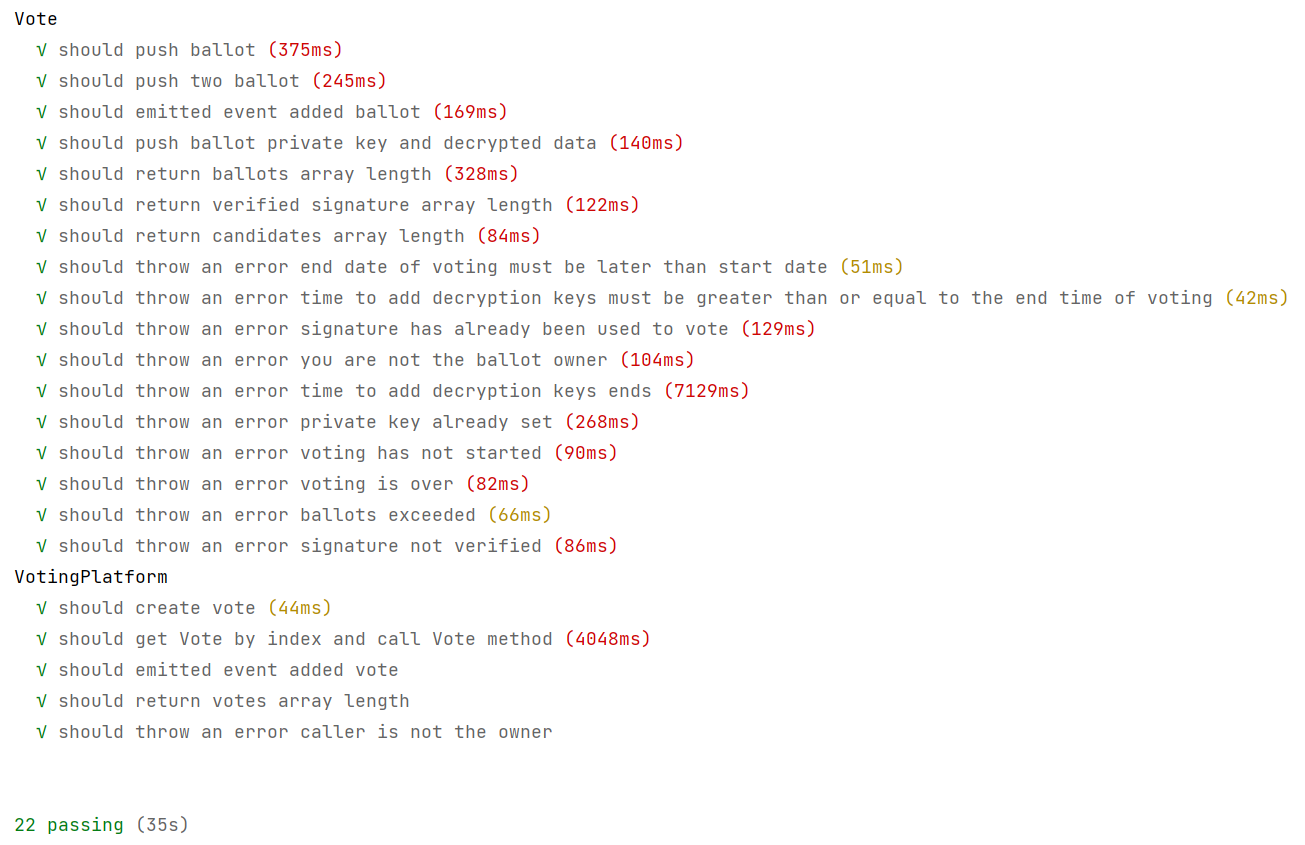
\includegraphics[width=1.0\hsize]{fig/unit-tests.png}\\[2mm]
\caption{Выполнение модульных тестов}\label{fig:unittest}
\end{center}
\end{figure}

\begin{figure}[H]
\begin{center}
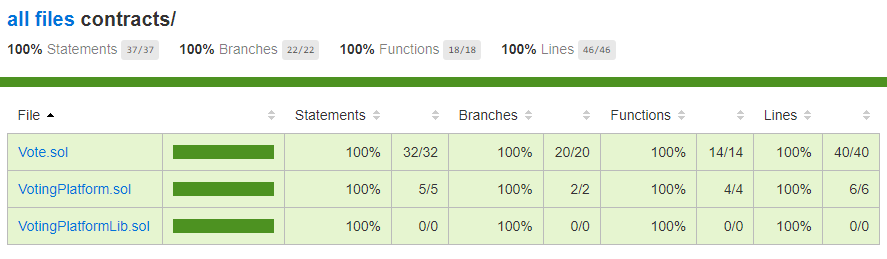
\includegraphics[width=1.0\hsize]{fig/coverage.png}\\[2mm]
\caption{Статистика покрытия кодовой базы}\label{fig:coverage}
\end{center}
\end{figure}